\documentclass[10pt,a4paper]{article}

% --- Core Packages ---
\usepackage[utf8]{inputenc}
\usepackage[T1]{fontenc}
\usepackage{helvet}
\renewcommand{\familydefault}{\sfdefault}
\usepackage{microtype}
\usepackage[margin=0.6in, top=0.6in, bottom=0.6in]{geometry}
\usepackage[table]{xcolor}
\usepackage{amsmath,amssymb}
\usepackage{booktabs}
\usepackage{tabularx}
\usepackage{graphicx}
\usepackage{multirow}
\usepackage{array}
\usepackage{enumitem}
\usepackage{tcolorbox}
\tcbuselibrary{skins,breakable}
\usepackage{tikz}
\usetikzlibrary{positioning,calc,shapes.geometric,backgrounds,patterns}
\usepackage{fontawesome5}
\usepackage{titlesec}
\usepackage{fancyhdr}
\usepackage{lastpage}
\usepackage[hidelinks,pdfencoding=auto,psdextra]{hyperref}

% --- Color Palette ---
\definecolor{PrimaryNavy}{HTML}{0F2C59}   % Deep clinical navy
\definecolor{SecondaryTeal}{HTML}{1E6B7B} % Medical teal
\definecolor{AccentCoral}{HTML}{D9534F}   % Alert/Highlight coral
\definecolor{BgSlate}{HTML}{F4F7F9}       % Soft gray-blue background
\definecolor{BorderGray}{HTML}{D0D7DE}    % Subtle divider gray
\definecolor{TextDark}{HTML}{222222}      % Soft black for text
\definecolor{HeaderBg}{HTML}{E8F1F5}      % Table header background

% --- Page Setup & Headers ---
\pagestyle{fancy}
\fancyhf{}
\renewcommand{\headrulewidth}{0.4pt}
\renewcommand{\footrulewidth}{0.4pt}
\setlength{\headheight}{14pt}

\lhead{\small \color{SecondaryTeal}\textbf{GRANT APPLICATION: MER-2026-CRG-8841}}
\rhead{\small \color{PrimaryNavy}\textbf{Vertex Academic Medical Center}}
\lfoot{\small \color{gray}Confidential --- Meridian Foundation Clinical Research Program}
\rfoot{\small \color{PrimaryNavy}\textbf{Page \thepage\ of \pageref{LastPage}}}

% --- Typography & Section Formats ---
\titleformat{\section}
  {\color{PrimaryNavy}\Large\bfseries}
  {\thesection.}
  {0.5em}
  {}
  [\vspace{0.1em}\color{SecondaryTeal}\hrule height 1.2pt]

\titleformat{\subsection}
  {\color{SecondaryTeal}\large\bfseries}
  {\thesubsection}
  {0.5em}
  {}

\titleformat{\subsubsection}
  {\color{PrimaryNavy}\normalsize\bfseries}
  {\thesubsubsection}
  {0.5em}
  {}

\titlespacing*{\section}{0pt}{0.6em}{0.2em}
\titlespacing*{\subsection}{0pt}{0.5em}{0.2em}
\titlespacing*{\subsubsection}{0pt}{0.4em}{0.15em}

\setlength{\parskip}{0.3em}
\setlength{\parindent}{0pt}

% --- TColorBox Styles ---
\tcbset{
  grantbox/.style={
    enhanced,
    colback=BgSlate,
    colframe=PrimaryNavy,
    arc=3pt,
    boxrule=1pt,
    left=8pt, right=8pt, top=5pt, bottom=5pt
  },
  summarybox/.style={
    enhanced,
    colback=HeaderBg,
    colframe=SecondaryTeal,
    arc=2pt,
    boxrule=0.8pt,
    left=8pt, right=8pt, top=4pt, bottom=4pt
  },
  ethicalbox/.style={
    enhanced,
    colback=white,
    colframe=PrimaryNavy,
    arc=2pt,
    boxrule=0.8pt,
    left=8pt, right=8pt, top=4pt, bottom=4pt
  }
}

\begin{document}

% ==========================================
% GRANT APPLICATION HEADER / METADATA BLOCK
% ==========================================
\begin{tcolorbox}[grantbox]
\begin{center}
  {\small \color{SecondaryTeal}\textbf{\faFlask\ MERIDIAN FOUNDATION CLINICAL INVESTIGATOR GRANT PROGRAM (FY2026--2029)}} \\[0.2em]
  {\Large \color{PrimaryNavy}\textbf{Targeted Nanoparticle Immunotherapy in Refractory Triple-Negative Breast Cancer: Phase IIa Clinical Trial \& Biomarker Cohort Analysis}} \\[0.3em]
  \color{BorderGray}\hrule height 0.8pt \vspace{0.3em}
\end{center}

\begin{minipage}[t]{0.48\textwidth}
  \small
  \textbf{\color{PrimaryNavy}Principal Investigator:} Dr. Evelyn Reed, MD, PhD \\
  \textbf{Title:} Director of Translational Oncology \\
  \textbf{Institution:} Vertex Academic Medical Center \\
  \textbf{Email:} e.reed@vertex-med.org \quad \textbf{Phone:} +1 (555) 019-2834 \\[0.2em]
  \textbf{\color{PrimaryNavy}Co-Investigators:} \\
  --- Dr. Marcus Vance, PhD (Synapse Bioinformatics Institute) \\
  --- Dr. Sarah Jenkins, MD (Nexa Research Health Network)
\end{minipage}%
\hfill
\begin{minipage}[t]{0.48\textwidth}
  \small
  \textbf{\color{PrimaryNavy}Funding Opportunity Announcement:} MER-2026-CRG-8841 \\
  \textbf{\color{PrimaryNavy}Proposed Project Period:} Oct 1, 2026 --- Sep 30, 2029 (36 Months) \\
  \textbf{\color{PrimaryNavy}Total Requested Budget:} \$1,850,000 USD \\
  \textbf{\color{PrimaryNavy}IRB Approval Status:} Approved (\#2026-VAMC-0492) \\
  \textbf{\color{PrimaryNavy}FDA IND Status:} Active (IND \#168,402) \\
  \textbf{\color{PrimaryNavy}Primary Study Site:} Vertex Clinical Research Center
\end{minipage}
\end{tcolorbox}

% ==========================================
% SECTION 1: PROJECT SUMMARY & SPECIFIC AIMS
% ==========================================
\section{Project Summary \& Specific Aims}

\subsection{Executive Summary}
\begin{tcolorbox}[summarybox]
\textbf{\color{SecondaryTeal}Project Synopsis:} Triple-Negative Breast Cancer (TNBC) accounts for 15--20\% of all invasive breast carcinomas and exhibits disproportionate mortality due to rapid disease progression, early metastatic recurrence, and a lack of targeted therapeutic options. While immune checkpoint blockade (ICB) has improved outcomes in PD-L1-positive disease, over 65\% of refractory TNBC patients fail to achieve durable clinical responses. This proposal presents a multi-center Phase IIa clinical trial investigating \textbf{Nexa-NP402}---a novel lipid-polymer nanoparticle encapsulating STING agonists alongside anti-PD-1 monoclonal antibodies. By converting immunologically ``cold'' tumor microenvironments into highly inflamed ``hot'' sites, this intervention aims to overcome primary therapeutic resistance. Supported by robust preliminary pre-clinical data from Synapse Bio, this 3-year study evaluates clinical efficacy, rigorous patient cohort power modeling, and longitudinal single-cell spatial transcriptomics in 96 stratified patients.
\end{tcolorbox}

\subsection{Background \& Clinical Rationale}
Metastatic TNBC carries a dismal 5-year overall survival rate of under 12\%. Current standard-of-care regimens relying on systemic platinum-based chemotherapy yield transient responses burdened by severe cumulative toxicity. Recent clinical trials demonstrate that monotherapy with anti-PD-1 agents achieves objective response rates (ORR) of only 10--15\% in unselected refractory populations. The primary mechanistic bottleneck is the immunosuppressive tumor microenvironment (TME), characterized by dense tumor stroma, defective antigen presentation, and a scarcity of tumor-infiltrating CD8+ T lymphocytes.

\textbf{Nexa-NP402} is engineered to target tumor-associated macrophages (TAMs) via mannose-receptor endocytosis, delivering localized cyclic dinucleotides (STING agonists) while simultaneously blocking the PD-1/PD-L1 axis. In preliminary murine models conducted at Vertex AMC, Nexa-NP402 elicited complete tumor regression in 58\% of subjects and established long-term immunological memory without inducing systemic cytokine release syndrome.

\subsection{Hypothesis \& Specific Aims}
We hypothesize that co-administration of Nexa-NP402 with pembrolizumab will significantly prolong progression-free survival (PFS) in patients with refractory TNBC by reprogramming the TME and driving clonal expansion of tumor-reactive T cells.

\begin{description}[font=\color{PrimaryNavy}\bfseries, leftmargin=1.2em, itemsep=0.15em]
  \item[\lbrack Aim 1\rbrack Phase IIa Clinical Efficacy \& Safety Evaluation:] Conduct an open-label, randomized 1:1 Phase IIa trial ($N=96$) comparing Nexa-NP402 + pembrolizumab against physician's choice single-agent chemotherapy. Primary endpoint: Progression-Free Survival (PFS) at 12 months. Secondary endpoints: Overall Response Rate (ORR) per RECIST v1.1 and safety profile per CTCAE v5.0.
  
  \item[\lbrack Aim 2\rbrack Patient Cohort Power Analysis \& Biomarker Profiling:] Perform high-dimensional single-cell RNA sequencing (scRNA-seq) and spatial transcriptomics on pre- and post-treatment core biopsies. Evaluate baseline immune signatures, interferon-gamma gene response scores, and somatic mutation burden as predictive biomarkers of response.
  
  \item[\lbrack Aim 3\rbrack Pharmacokinetics \& Circulating Tumor DNA (ctDNA) Dynamics:] Track serial liquid biopsies at baseline, Week 2, Week 6, and progression to quantify ctDNA clearance kinetics using custom targeted ultra-deep sequencing, correlating clearance rates with durable clinical benefit.
\end{description}

% ==========================================
% SECTION 2: STUDY DESIGN & POWER ANALYSIS
% ==========================================
\section{Study Design \& Patient Cohort Power Analysis}

\subsection{Clinical Trial Architecture}
The trial utilizes a prospective, randomized, open-label Phase IIa design across two primary clinical sites (Vertex Academic Medical Center and Nexa Health Network). Patient enrollment will proceed over 18 months, followed by 18 months of active treatment and longitudinal follow-up.

\begin{center}
\begin{tcolorbox}[colback=white,colframe=BorderGray,arc=2pt,boxrule=0.5pt,left=4pt,right=4pt,top=4pt,bottom=4pt]
\centering
\resizebox{0.96\textwidth}{!}{%
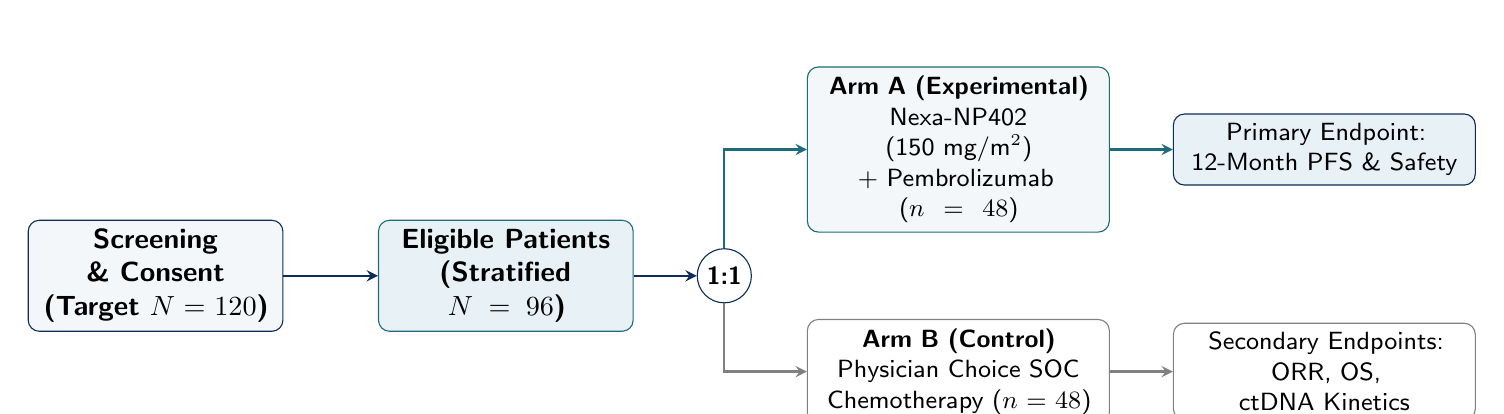
\begin{tikzpicture}[node distance=0.8cm and 1.2cm, auto, >=stealth, every node/.style={font=\small}]
  % Nodes
  \node [draw=PrimaryNavy, fill=BgSlate, rounded corners, rectangle, text width=3.0cm, align=center, font=\bfseries] (screen) {Screening \& Consent\\(Target $N=120$)};
  \node [draw=SecondaryTeal, fill=HeaderBg, rounded corners, rectangle, text width=3.0cm, align=center, right=of screen, font=\bfseries] (eligible) {Eligible Patients\\(Stratified $N=96$)};
  \node [draw=PrimaryNavy, circle, inner sep=2pt, right=0.8cm of eligible, font=\bfseries\small] (rand) {1:1};
  \node [draw=SecondaryTeal, fill=BgSlate, rounded corners, rectangle, text width=3.6cm, align=center, above right=0.3cm and 0.8cm of rand] (armA) {\textbf{Arm A (Experimental)}\\Nexa-NP402 (150 mg/m$^2$)\\+ Pembrolizumab ($n=48$)};
  \node [draw=gray, fill=white, rounded corners, rectangle, text width=3.6cm, align=center, below right=0.3cm and 0.8cm of rand] (armB) {\textbf{Arm B (Control)}\\Physician Choice SOC\\Chemotherapy ($n=48$)};
  \node [draw=PrimaryNavy, fill=HeaderBg, rounded corners, rectangle, text width=3.6cm, align=center, right=0.8cm of armA] (endA) {Primary Endpoint:\\12-Month PFS \& Safety};
  \node [draw=gray, fill=white, rounded corners, rectangle, text width=3.6cm, align=center, right=0.8cm of armB] (endB) {Secondary Endpoints:\\ORR, OS, ctDNA Kinetics};

  % Paths
  \draw [->, thick, PrimaryNavy] (screen) -- (eligible);
  \draw [->, thick, PrimaryNavy] (eligible) -- (rand);
  \draw [->, thick, SecondaryTeal] (rand) |- (armA);
  \draw [->, thick, gray] (rand) |- (armB);
  \draw [->, thick, SecondaryTeal] (armA) -- (endA);
  \draw [->, thick, gray] (armB) -- (endB);
\end{tikzpicture}%
}
\end{tcolorbox}
\end{center}

\begin{table}[htbp]
\caption{\textbf{Patient Eligibility Criteria}}
\vspace{-0.4em}
\small
\begin{tabularx}{\textwidth}{X X}
\toprule
\rowcolor{HeaderBg} \textbf{\color{PrimaryNavy}Inclusion Criteria} & \textbf{\color{PrimaryNavy}Exclusion Criteria} \\
\midrule
1. Histologically confirmed unresectable or metastatic TNBC. & 1. Active symptomatic brain metastases or leptomeningeal disease. \\
2. Prior treatment with $\ge 1$ systemic chemotherapy regimen. & 2. Prior exposure to STING agonist therapies. \\
3. ECOG Performance Status 0 or 1. & 3. Active autoimmune disease requiring systemic immunosuppression. \\
4. Measurable disease per RECIST v1.1 criteria. & 4. Inadequate organ function (ALT/AST $> 2.5\times$ ULN; CrCl $< 45$ mL/min). \\
5. Fresh tumor biopsy feasible at baseline and Week 6. & 5. Prolonged QTc interval ($> 470$ ms). \\
\bottomrule
\end{tabularx}
\end{table}

\subsection{Patient Cohort Power Analysis \& Sample Size Calculations}
Statistical power modeling was conducted to ensure sufficient sample size to detect a clinically meaningful improvement in median PFS. Historical data for standard-of-care chemotherapy in second-line metastatic TNBC indicate a median PFS of 4.2 months. We hypothesize that Nexa-NP402 + pembrolizumab will extend median PFS to 7.0 months, corresponding to a hazard ratio ($\text{HR}$) of 0.60.

Sample size calculations were executed using the Schoenfeld formula for Cox proportional hazards regression:
\begin{equation}
  E = \frac{4 \, (z_{\alpha/2} + z_{1-\beta})^2}{(\ln \text{HR})^2}
\end{equation}

Where:
\begin{itemize}[leftmargin=1.5em, topsep=1pt, itemsep=1pt]
  \item $E$ is the required total number of progression events.
  \item $\alpha = 0.05$ (two-sided type I error rate, $z_{\alpha/2} = 1.960$).
  \item $1-\beta = 0.85$ (statistical power of 85\%, $z_{1-\beta} = 1.036$).
  \item $\text{HR} = 0.60$ (target hazard ratio, $\ln \text{HR} = -0.5108$).
\end{itemize}

Substituting the parameters into Equation (1):
\begin{equation}
  E = \frac{4 \times (1.960 + 1.036)^2}{(-0.5108)^2} = \frac{4 \times (2.996)^2}{0.2609} = \frac{35.904}{0.2609} \approx 138 \text{ total required events}
\end{equation}

Assuming a total accrual period of 18 months, a minimum follow-up of 18 months, and an expected exponential dropout rate of 5\% per annum, a sample size of $n = 48$ evaluable patients per arm ($N = 96$ total evaluable patients) yields 85.4\% power to reject the null hypothesis at $\alpha = 0.05$. To account for an anticipated 15\% non-evaluability rate (due to protocol violations or early consent withdrawal), target enrollment is set at $N = 113$ (rounded to $N = 120$ screened subjects).

\begin{table}[htbp]
\caption{\textbf{Cohort Stratification \& Statistical Power Parameters}}
\vspace{-0.4em}
\small
\begin{tabularx}{\textwidth}{l c c X c c}
\toprule
\rowcolor{HeaderBg} \textbf{Cohort Subgroup} & \textbf{Target $n$} & \textbf{PD-L1 Status} & \textbf{Primary Endpoint} & \textbf{Effect Size} & \textbf{Power ($\alpha=0.05$)} \\
\midrule
\textbf{Cohort A1 (Arm A)} & 28 & CPS $\ge 10$ & PFS \& ORR & $\text{HR} = 0.52$ & 88.2\% \\
\textbf{Cohort A2 (Arm A)} & 20 & CPS $< 10$ & PFS \& Immune Activation & $\text{HR} = 0.65$ & 81.5\% \\
\textbf{Cohort B1 (Arm B)} & 28 & CPS $\ge 10$ & PFS (Standard SOC) & Baseline & Reference \\
\textbf{Cohort B2 (Arm B)} & 20 & CPS $< 10$ & PFS (Standard SOC) & Baseline & Reference \\
\midrule
\textbf{Total Evaluable} & \textbf{96} & --- & \textbf{12-Month PFS} & \textbf{$\text{HR} = 0.60$} & \textbf{85.4\%} \\
\bottomrule
\end{tabularx}
\end{table}

% ==========================================
% SECTION 3: ETHICAL APPROVAL & GOVERNANCE
% ==========================================
\section{Ethical Approval, Patient Safety \& Regulatory Compliance}

\subsection{Institutional Review Board (IRB) \& Regulatory Authorizations}
This protocol has undergone full committee review and received formal approval from the Vertex Academic Medical Center Institutional Review Board (Protocol ID: \textbf{IRB-2026-VAMC-0492}, Approved June 12, 2026). The investigation will be conducted in strict compliance with the Declaration of Helsinki, the International Council for Harmonisation (ICH) Good Clinical Practice (GCP) guidelines (E6 R2), and applicable US FDA regulations (21 CFR Parts 50, 56, and 312).

An Investigational New Drug (IND) application for Nexa-NP402 was submitted to the US FDA and declared active under \textbf{IND \#168,402}.

\subsection{Patient Informed Consent \& Data Privacy Framework}
Written informed consent will be obtained from all participants prior to any study-mandated procedures. The consent document explicitly details potential risks, including immune-related adverse events (irAEs), biopsy risks, and optional participation in exploratory genomic assays.

\begin{tcolorbox}[ethicalbox]
\textbf{\color{PrimaryNavy}\faLock\ Data Protection \& HIPAA Compliance Specifications:}
\begin{itemize}[leftmargin=1.5em, topsep=1pt, itemsep=1.5pt]
  \item \textbf{De-Identification:} All patient specimens and digital clinical metrics will be pseudo-anonymized using 128-bit hash identifiers (UUIDv4) in compliance with the HIPAA Safe Harbor standard (45 CFR \S 164.514).
  \item \textbf{Genomic Privacy:} Whole-exome and scRNA-seq datasets will be stored within an isolated, SOC2-certified cloud infrastructure managed by Synapse Bio. Raw genomic data access will be restricted to named investigators.
  \item \textbf{Biobank Governance:} Leftover tissue and blood fractions will be archived at the Vertex Biobank with strict patient opt-in rights for future secondary research.
\end{itemize}
\end{tcolorbox}

\subsection{Data Safety Monitoring Board (DSMB) Charter}
An independent Data Safety Monitoring Board (DSMB) comprising two medical oncologists, one biostatistician, and an independent patient advocate will oversee patient safety. The DSMB will convene after enrollment of every 24 patients or upon occurrence of any Grade $\ge 4$ treatment-related adverse event.

\textbf{Interim Stopping Rules:} Formal interim analyses for efficacy and futility will occur when 46 and 92 PFS events are observed, utilizing O'Brien-Fleming group sequential boundaries. The trial may be terminated early for efficacy if the two-sided $p$-value falls below $0.003$ at the first interim review.

% ==========================================
% SECTION 4: MILESTONES & WORK PACKAGES
% ==========================================
\section{Research Implementation, Milestones \& Risk Management}

\subsection{Work Package Structure}
The 36-month project is structured into four integrated Work Packages (WPs) executed collaboratively across Vertex AMC, Synapse Bio, and Nexa Health.

\begin{table}[htbp]
\caption{\textbf{Work Package Breakdown \& Milestones}}
\vspace{-0.4em}
\small
\begin{tabularx}{\textwidth}{c X c c l}
\toprule
\rowcolor{HeaderBg} \textbf{WP \#} & \textbf{Work Package Title} & \textbf{Lead Site} & \textbf{Period} & \textbf{Key Deliverables / Milestones} \\
\midrule
\textbf{WP1} & Clinical Trial Setup \& Site Activation & Vertex AMC & M01--M06 & Site IRB greenlight; 100\% supply of Nexa-NP402. \\
\textbf{WP2} & Patient Recruitment \& Phase IIa Trial & Nexa Health & M06--M28 & Complete recruitment ($N=120$); 12-month PFS endpoint. \\
\textbf{WP3} & Single-Cell Transcriptomics \& Profiling & Synapse Bio & M12--M30 & Complete scRNA-seq on 192 paired tissue biopsies. \\
\textbf{WP4} & Integrated Biomarker \& ctDNA Modeling & Vertex AMC & M24--M36 & Final statistical synthesis; FDA Phase III meeting. \\
\bottomrule
\end{tabularx}
\end{table}

\subsection{Risk Assessment \& Mitigation Framework}

\begin{table}[htbp]
\caption{\textbf{Risk Matrix and Contingency Planning}}
\vspace{-0.4em}
\small
\begin{tabularx}{\textwidth}{X c c X}
\toprule
\rowcolor{HeaderBg} \textbf{Identified Risk Factor} & \textbf{Severity} & \textbf{Likelihood} & \textbf{Mitigation Strategy} \\
\midrule
Slow patient accrual rate ($<4$ patients/month) & High & Moderate & Activate 2 additional secondary community oncology sites within Nexa Health Network. \\
Severe immune-related adverse events (Grade $\ge 3$ irAEs) & High & Low & Enforce strict dose-reduction algorithm; immediate administration of high-dose corticosteroids. \\
Biopsy tissue degradation / low RNA yield & Moderate & Low & Standardize snap-freezing protocols; utilize low-input RNA-seq library preparation kits. \\
High loss-to-follow-up rate ($>15\%$) & Moderate & Moderate & Patient travel stipends; telehealth safety check-ins at alternating bi-weekly intervals. \\
\bottomrule
\end{tabularx}
\end{table}

% ==========================================
% SECTION 5: BUDGET & RESOURCE ALLOCATION
% ==========================================
\section{Detailed Budget \& Resource Justification}

\subsection{Budget Summary}
The total requested budget for the 3-year project is \textbf{\$1,850,000 USD}. Indirect costs are calculated at the institutional negotiated rate of 14.2\% for clinical research activities.

\begin{table}[htbp]
\caption{\textbf{Project Budget Breakdown (USD)}}
\vspace{-0.4em}
\small
\begin{tabularx}{\textwidth}{X r r r r}
\toprule
\rowcolor{HeaderBg} \textbf{Cost Category} & \textbf{Year 1 (\$)} & \textbf{Year 2 (\$)} & \textbf{Year 3 (\$)} & \textbf{Total (\$)} \\
\midrule
\textbf{Personnel} (PI, Co-Is, Clinical Coordinators, Bioinformatician) & 245,000 & 255,000 & 265,000 & 765,000 \\
\textbf{Clinical Trial Operational Costs} (Pharmacy, Imaging, IRB) & 180,000 & 160,000 & 90,000 & 430,000 \\
\textbf{Laboratory \& Omics Assays} (scRNA-seq, ctDNA, Reagents) & 140,000 & 150,000 & 60,000 & 350,000 \\
\textbf{Patient Care \& Travel Compensation} & 25,000 & 30,000 & 20,000 & 75,000 \\
\midrule
\textbf{Direct Costs Subtotal} & \textbf{590,000} & \textbf{595,000} & \textbf{435,000} & \textbf{1,620,000} \\
\textbf{Indirect Costs} (14.2\% institutional rate) & 83,000 & 84,000 & 63,000 & 230,000 \\
\midrule
\rowcolor{HeaderBg} \textbf{\color{PrimaryNavy}Total Requested Budget} & \textbf{673,000} & \textbf{679,000} & \textbf{498,000} & \textbf{\$1,850,000} \\
\bottomrule
\end{tabularx}
\end{table}

\subsection{Budget Justification Narrative}
\textbf{Personnel (\$765,000):} Funds support PI Dr. Evelyn Reed (20\% effort), Co-PI Dr. Marcus Vance (15\% effort), two full-time Clinical Research Coordinators for patient tracking and data entry, and a 1.0 FTE Senior Bioinformatician at Synapse Bio dedicated to scRNA-seq and spatial transcriptomics analysis.

\textbf{Laboratory \& Omics Assays (\$350,000):} Direct sequencing costs for 192 paired tissue samples (scRNA-seq on Illumina NovaSeq 6000 at \$1,200/sample) and longitudinal ctDNA panel assays across 4 timepoints per patient (\$450/panel).

\vspace{0.4em}

% ==========================================
% SIGNATURE & ENDORSEMENT BLOCK
% ==========================================
\begin{center}
\begin{tcolorbox}[colback=white,colframe=PrimaryNavy,arc=2pt,boxrule=0.8pt,width=\textwidth]
\small
\textbf{\color{PrimaryNavy}INSTITUTIONAL ENDORSEMENT \& APPLICANT SIGNATURES} \\[0.2em]
We, the undersigned, certify that the statements herein are true, complete, and accurate to the best of our knowledge. The institution agrees to accept accountability for the scientific, ethical, and financial conduct of the project if awarded.

\vspace{0.8em}

\begin{minipage}[t]{0.45\textwidth}
  \color{PrimaryNavy}\hrule height 0.8pt \vspace{0.3em}
  \textbf{Dr. Evelyn Reed, MD, PhD} \\
  Principal Investigator \\
  Director of Translational Oncology, Vertex AMC \\
  Date: July 24, 2026
\end{minipage}%
\hfill
\begin{minipage}[t]{0.45\textwidth}
  \color{PrimaryNavy}\hrule height 0.8pt \vspace{0.3em}
  \textbf{Dr. Arthur Pendelton, MD} \\
  Dean of Clinical Research \& Authorized Official \\
  Vertex Academic Medical Center \\
  Date: July 24, 2026
\end{minipage}
\end{tcolorbox}
\end{center}

\end{document}
